\documentclass{article}

\usepackage{minitoc}
\usepackage{tabularx,setspace}
\usepackage{booktabs}
\usepackage{graphicx}
\usepackage{hyperref}
\usepackage{xcolor}
\usepackage{blkarray}
\usepackage{amsthm, amssymb, amsmath}
\usepackage{caption}
\usepackage{subcaption}
\usepackage{multirow}
\usepackage[ruled,vlined]{algorithm2e}

\usepackage{natbib}
\bibliographystyle{abbrvnat}

\theoremstyle{definition}
\newtheorem{definition}{Definition}[section]
\newtheorem{theorem}{Theorem}[section]
\newtheorem{lemma}[theorem]{Lemma}
\newtheorem{conjecture}[theorem]{Conjecture}

\usepackage[margin=2.5cm, includefoot, footskip=0pt]{geometry}
%\pagestyle{plain}
%\setlength{\parindent}{0em}
%\setlength{\parskip}{1em}

\renewcommand{\baselinestretch}{1}

\newcommand{\nikoleta}[1]{\textcolor{teal}{{\bf NG:} #1}}

\newtheorem{proposition}{Proposition}

\title{\vspace{-2cm} Good strategies with $n$-bit memory}

\author{Nikoleta E. Glynatsi, Christian Hilbe, Martin Nowak}
\date{}

\begin{document}

\maketitle

\onehalfspacing

\noindent
We are interested in extending the results of \citep{akin:EGADS:2016} to strategy spaces with $n\!>\!1$ rounds of memory. 
In the following, we outline our setup and our main conjecture so far.\\

\noindent
{\bf Repeated donation game.} We consider the infinitely repeated games among two players, player $p$ and player $q$. 
Each round, they engage in the donation game with payoff matrix
\begin{equation} \label{Eq:DonationGame}
\left(
\begin{array}{cc}
b-c	&-c\\
b	&0
\end{array}
\right).
\end{equation}
Here $b$ and $c$ denote the benefit and the cost of cooperation, respectively. 
We assume $b\!>\!c\!>\!0$ throughout. 
Therefore, the payoff matrix~\eqref{Eq:DonationGame} is a special case of a prisoner's dilemma.\\

\noindent
{\bf Memory-$n$ strategies.} We assume in the following, that the players' decisions only depend on the outcome of the previous $n$ rounds. 
To this end, an {\it $n$-history for player $p$} is a string $h^p=(a^p_{-1},\ldots,a^p_{-n})\!\in\!\{C,D\}^n$. 
An entry $a^p_{-k}$ corresponds to player $p$'s action $k$ rounds ago. 
Let $H^p$ denote the space of all $n$-histories of player~$p$. 
Analogously, we define $H^q$ as the set of $n$-histories $h^q$ of player~$q$. 
A pair $h\!=\!(h^p,h^q)$ is called an {\it $n$-history of the game}. 
We use $H=H^p\times H^q$ to denote the space of all such histories. 
This set contains $|H|=2^{2n}$ elements. 
A {\it memory-$n$} strategy is a vector $\mathbf{p}=(p_h)_{h\in H}\in[0,1]^{2^{2n}}$. 
Each entry $p_h$ corresponds to the player's cooperation probability in the next round, depending on the outcome of the previous $n$ rounds. 
One special case of such a memory-$n$ strategy is the  {\it round-$k$-repeat strategy} for some $1\!\le\!k\!\le\!n$. 
Player $p$ uses a {\it round-$k$-repeat strategy} $\mathbf{p}^{k-\text{Rep}}$ if in any given round, the player chooses the same action as $k$ rounds ago. That is, if the game's $n$-history is such that $a^p_{-k}\!=\!C$, then $p^{k-\text{Rep}}_h\!=\!1$; otherwise $p^{k-\text{Rep}}_h\!=\!0$.


If the two players use memory-$n$ strategies $\mathbf{p}$ and $\mathbf{q}$, one can represent the interaction as a Markov chain with a $2^{2n}\!\times\!2^{2n}$ transition matrix $M$. 
Let $\mathbf{v}=(v_h)_{h\in H}$ be an invariant distribution of this Markov chain. 
With the same method as in \citep{akin:EGADS:2016}, one can show {\it Akin's Lemma}: For each $k$ with $1\!\le\!k\!\le\!n$, the invariant distribution $\mathbf{v}$ satisfies the following relationship,
\begin{equation} \label{Eq:AkinsLemma}
\mathbf{v} \cdot (\mathbf{p}-\mathbf{p}^{k-\text{Rep}}) \!=\! \sum_{h\in H} v_h (p_h-p_h^{k-\text{Rep}}) = 0.
\end{equation}
The intuition for this result is that $\mathbf{v}\cdot \mathbf{p}$ and all $\mathbf{v}\cdot \mathbf{p}^{k-\text{Rep}}$ are just different (but equivalent) expressions for player $p$'s average cooperation rate. For example, $\mathbf{v}\cdot\mathbf{p}$ corresponds to a setup in which one first draws a history $h$ according to the invariant distribution $\mathbf{v}$; then one takes player $p$'s probability $p_h$ to cooperate in the next round; the expectation of this procedure is $\sum_{h\in H} v_h p_h$.

Based on the invariant distribution $\mathbf{v}$, we can also compute the players' payoffs. To this end, let $\mathbf{S}^k = (S_h^k)_{h\in H}$ denote the vector that returns for each $h$ the one-shot payoff that player $p$ obtained $k$ rounds ago, 
\begin{equation}
S_h^k = \left\{
\begin{array}{cl}
b-c	&\text{if}~ a_{-k}^p=C~\text{and}~ a_{-k}^q=C\\
-c	&\text{if}~ a_{-k}^p=C~\text{and}~ a_{-k}^q=D\\
b	&\text{if}~ a_{-k}^p=D~\text{and}~ a_{-k}^q=C\\
0	&\text{if}~ a_{-k}^p=D~\text{and}~ a_{-k}^q=D
\end{array}
\right.
\end{equation}
Then we can define player $p$'s repeated-game payoff $s_\mathbf{p}$ as 
\begin{equation} \label{Eq:Payoff}
s_\mathbf{p} = \mathbf{v}\cdot \mathbf{S}^1 = \mathbf{v}\cdot \mathbf{S}^2 = \ldots = \mathbf{v} \cdot \mathbf{S}^n.
\end{equation}
The equalities $ \mathbf{v}\cdot \mathbf{S}^1 = \ldots = \mathbf{v} \cdot \mathbf{S}^n$ correspond to the intuition that it does not matter which of the past $n$ rounds we use to define average payoffs (this is a direct consequence of Akin's Lemma). 
The payoff $s_\mathbf{q}$ of player $q$ can be defined analogously. 

Akin's lemma imposes some natural restrictions on which invariant distributions $\mathbf{v}$ are possible. Similar to the paper by \citep{akin:EGADS:2016}, we hope to exploit these restrictions to characterise the good memory-$n$ strategies (to be defined below).\\

\noindent
{\bf Good strategies.} 
We say $h\!=\!(h^p,h^q)$ is the mutual cooperation history if $h^p\!=\!h^q\!=\!(C,\ldots,C)$. 
A memory-$n$ strategy $\mathbf{p}$ is called agreeable if it prescribes to cooperate with probability 1 after the mutual cooperation history. 
The strategy $\mathbf{p}$ is called good if it is agreeable and if expected payoffs satisfy
\begin{equation} \label{Eq:good}
    s_{\mathbf{q}} \geq b\!-\!c \qquad \Rightarrow \qquad s_{\mathbf{q}} = s_{\mathbf{p}} =  b\!-\!c.
\end{equation}
We wish to characterise all good memory-$n$ strategies of the repeated donation game. To start with, in the following we begin with the simplest non-trivial case.\\

\noindent
{\bf The case of 2-bit reactive strategies.} 
We say a memory-$n$ strategy $\mathbf{p}$ is {\it $n$-bit reactive} if it only depends on the co-player's $n$-history (independent of the focal player's own actions during the past $n$ rounds). Formally, $\mathbf{p}\!=\!(p_h)_{h \in H}$ is $n$-bit reactive if for any two histories $h=(h^p,h^q)$ and $\tilde{h}=(\tilde{h}^p,\tilde{h}^q)$ with $h^q=\tilde{h}^q$ it follows that $p_h = p_{\tilde{h}}$. In particular, for $n\!=\!2$ such a player uses at most 4 different cooperation probabilities, depending on the co-player's actions during the last 2 rounds ($CC, CD, DC, DD$, where the first letter refers to the co-player's action in the second-to-last round, and the second letter refers to the last round). Slightly abusing notation, we write 2-bit reactive strategies as 
\begin{equation}
\mathbf{\hat{p}} = (\hat{p}_{CC}, \hat{p}_{CD}, \hat{p}_{DC}, \hat{p}_{DD}). 
\end{equation}
For 2-bit reactive strategies, we have the following conjecture.\\

\noindent
{\bf Conjecture.}
Let $\mathbf{\hat{p}}$ be an agreeable 2-bit reactive strategy, i.e. $\hat{p}_{CC}\!=\!1$. The following are equivalent\\[-0.7cm]
\begin{description} \setlength\itemsep{0pt}
\item[({\it i})] The strategy $\mathbf{\hat{p}}$ is good.
\item[({\it ii})] The entries of $\mathbf{\hat{p}}$ satisfy $\displaystyle \hat{p}_{DD} < 1\!-\! \frac{c}{b}$  ~~and~~ $\displaystyle \frac{\hat{p}_{CD} + \hat{p}_{DC}}{2} < 1-\frac{c}{2b}$.
\end{description}

~\\
Our evidence for this conjecture is as follows. The direction ({\it i}) $\Rightarrow$ ({\it ii}) is straightforward. If $\mathbf{p}$ is good, it needs to satisfy condition~\eqref{Eq:good} for all $\mathbf{q}$. In particular, the condition needs to be satisfied when $\mathbf{q}$ is either \emph{ALLD} (the strategy that always defects), or \emph{Alternator} (the strategy that cooperates if and only if it didn't cooperate the previous round). By checking these two strategies explicitly, one gets~({\it ii}). 

The direction  ({\it ii}) $\Rightarrow$ ({\it i}) we could not prove yet. However, we have strong numerical evidence (see Figure next page). We have sampled $10^4$ random agreeable 2-bit reactive strategies and checked numerically whether or not they are Nash equilibria. We found that exactly those strategies are Nash equilibria that satisfy the conditions in ({\it ii}).


\begin{figure}[t]
  \centering
  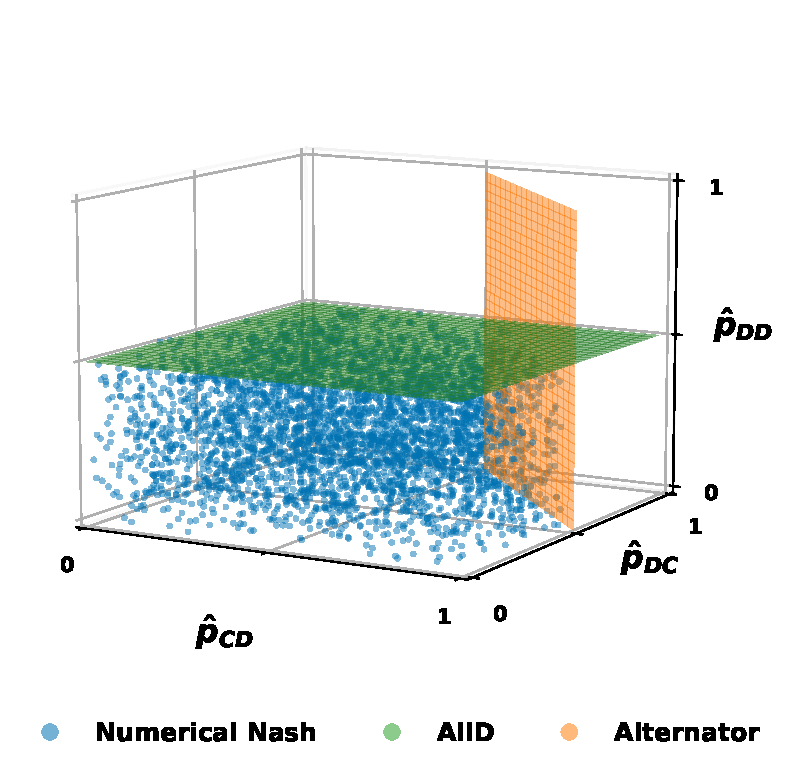
\includegraphics[width=.45\textwidth]{static/for_akin_no_proved_area.pdf}
  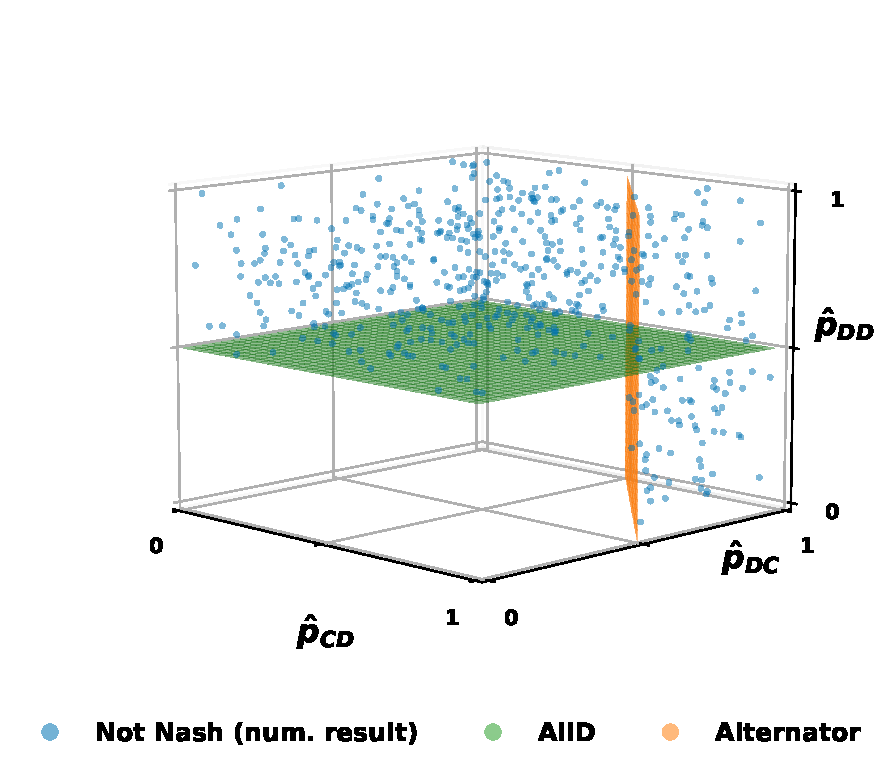
\includegraphics[width=.5\textwidth]{static/for_akin_non_nash.pdf}
  \caption{We generated $10^4$ agreeable 2-bit strategies of the form $\mathbf{\hat{p}}=(1,\hat{p}_{CD},\hat{p}_{DC},\hat{p}_{DD})$ uniformly at random. 
  For each such $\mathbf{\hat{p}}$ we numerically checked whether or not the strategy is a Nash equilibrium. 
  To this end, by an argument similar to the one in \citep{press:PNAS:2012} and  \citep{mcavoy:PRSA:2019}, it is sufficient to check all deviations towards pure memory-2 strategies $\mathbf{q}$.
  If a strategy $\mathbf{\hat{p}}$ was numerically found to be a Nash equilibrium, we depict it as a blue dot in the left panel.
  Otherwise, if it was found not to be a Nash equilibrium, we depict it as a blue dot in the right panel.  
  Points below the green plane satisfy $\hat{p}_{DD} < 1\!-\! \frac{c}{b}$. 
  Points left to the orange plane satisfy $\hat{p}_{CD} + \hat{p}_{DC} < 2-\frac{c}{b}$.
  We find that all Nash equilibria satisfy these two inequalities (left panel). 
  Conversely, our numerical results suggest that all $\mathbf{\hat{p}}$ that are not Nash equilibria violate at least one of these inequalities (right panel).
  Parameters: $b\!=\!2$, $c\!=\!1$.
  }
\end{figure}

~\\
\bibliography{bibliography.bib}

\end{document}